\documentclass[12pt,a4paper]{article}
\usepackage[utf8]{vietnam}
\usepackage{amsmath,amssymb}
\usepackage{tabularx}
\usepackage{tikz}
\usetikzlibrary{calc,angles,quotes,arrows.meta,patterns}
\usepackage{xcolor}
\usepackage{enumitem}
\usepackage{fancyhdr}
\usepackage[top=1.2cm, bottom=1.2cm, left=1.5cm, right=1.5cm]{geometry}
\usepackage[dethi]{ex_test}
\SAOPTN{widthSA=2.6,heightSA=0.62}

\setlength{\headheight}{15pt}
\setlength{\parskip}{0pt}

\pagestyle{fancy}
\fancyhf{}
\rhead{\textit{Môn Toán 6 -- Đề số 12}}
\lhead{\textit{Bộ đề ôn tập Giữa học kì I}}
\cfoot{\thepage}

\begin{document}

% --- KHUNG TIÊU ĐỀ ĐỀ THI ---
\noindent
\begin{tabularx}{\linewidth}{X r}
\textbf{TRƯỜNG THCS: \dotfill} & \textbf{ĐỀ KIỂM TRA ĐỊNH KỲ GIỮA HỌC KỲ I} \\
\textbf{Họ và tên: \dotfill} & \textbf{NĂM HỌC 2026 -- 2027} \\
\textbf{Lớp: \dotfill \quad SBD: \dotfill} & \textbf{Môn: TOÁN 6} \\
\hline
\end{tabularx}
\vspace{2mm}

\begin{center}
  \textbf{\large ĐỀ ÔN TẬP GIỮA HỌC KỲ I -- ĐỀ SỐ 12}\\
  \textit{Thời gian làm bài: 90 phút (Không kể thời gian phát đề)}
\end{center}
\vspace{1mm}

% --- PHẦN I ---
\noindent\textbf{\large PHẦN I. CÂU TRẮC NGHIỆM NHIỀU PHƯƠNG ÁN LỰA CHỌN (3,0 điểm)}

\textit{Thí sinh trả lời từ câu 1 đến câu 12. Mỗi câu hỏi thí sinh chỉ chọn một phương án duy nhất.}

\vspace{1mm}
\begin{ex}
Trong các số $1904; 2895; 2890; 2786$, số chia hết cho 5 mà không chia hết cho 2 là:
\choice
{$1904$}
{\True $2895$}
{$2890$}
{$2786$}
\end{ex}

\begin{ex}
Cho hình chữ nhật $ABCD$ có $AB = 5\text{ cm}, BC = 2\text{ cm}$ thì độ dài cạnh $CD$ là:
\choice
{$CD = 3\text{ cm}$}
{$CD = 2\text{ cm}$}
{\True $CD = 5\text{ cm}$}
{$CD = 7\text{ cm}$}
\end{ex}

\begin{ex}
Trong các số tự nhiên sau, số nào là số nguyên tố?
\choice
{$4$}
{$49$}
{\True $47$}
{$125$}
\end{ex}

\begin{ex}
Các ước nguyên tố của 12 là:
\choice
{$1; 2; 3$}
{\True $2; 3$}
{$2; 3; 4; 6$}
{$1; 2; 3; 4; 6; 12$}
\end{ex}

\begin{ex}
Phát biểu nào sau đây là sai?\\Trong một hình thang cân:
\choice
{Hai góc kề một đáy bằng nhau}
{Hai đường chéo bằng nhau}
{Hai cạnh bên bằng nhau}
{\True Các cạnh đối song song với nhau}
\end{ex}

\begin{ex}
Trong phép chia có dư, số dư bao giờ cũng \dots\dots số chia:
\choice
{\True Nhỏ hơn}
{Lớn hơn}
{Nhỏ hơn hoặc bằng}
{Lớn hơn hoặc bằng}
\end{ex}

\begin{ex}
Số 19 trong hệ La Mã được viết là:
\choice
{IX}
{IXX}
{XXI}
{\True XIX}
\end{ex}

\begin{ex}
Một hình vuông có diện tích bằng $121\text{ cm}^2$. Chu vi của hình vuông đó bằng:
\choice
{$22\text{ cm}$}
{$11\text{ cm}$}
{$48\text{ cm}$}
{\True $44\text{ cm}$}
\end{ex}

\begin{ex}
Một tấm biển quảng cáo hình chữ nhật có chiều dài $40\text{ dm}$, chiều rộng là $6\text{ dm}$. Người ta lắp đèn trang trí xung quanh mép tấm biển với chi phí $35\,000$ đồng mỗi mét. Số tiền phải chi cho việc mua đèn là:
\choice
{\True $420\,000$ đồng}
{$840\,000$ đồng}
{$322\,000$ đồng}
{$161\,000$ đồng}
\end{ex}

\begin{ex}
Trong các hình dưới đây, hình nào là hình lục giác đều?
\begin{center}
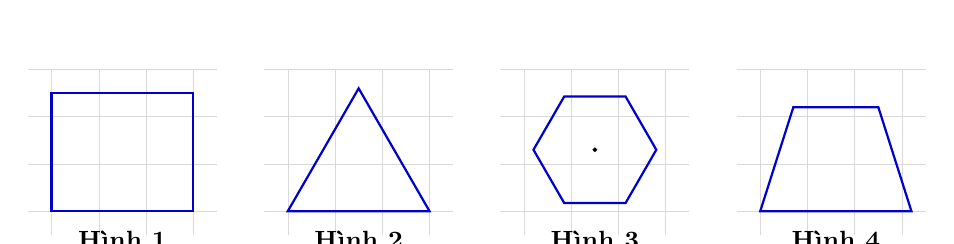
\begin{tikzpicture}[scale=0.6, font=\small]
  % Hinh 1: Hinh chu nhat
  \begin{scope}[shift={(0,0)}]
    \draw[help lines, gray!30] (-0.5,-0.5) grid (3.5,3);
    \draw[thick, blue!80!black] (0,0) rectangle (3,2.5);
    \node at (1.5, -0.6) {\textbf{Hình 1}};
  \end{scope}
  % Hinh 2: Tam giac
  \begin{scope}[shift={(5,0)}]
    \draw[help lines, gray!30] (-0.5,-0.5) grid (3.5,3);
    \draw[thick, blue!80!black] (0,0) -- (3,0) -- (1.5,2.6) -- cycle;
    \node at (1.5, -0.6) {\textbf{Hình 2}};
  \end{scope}
  % Hinh 3: Luc giac deu
  \begin{scope}[shift={(10,0)}]
    \draw[help lines, gray!30] (-0.5,-0.5) grid (3.5,3);
    \coordinate (O) at (1.5, 1.3);
    \foreach \a in {0,60,120,180,240,300} {
      \coordinate (P\a) at ($(O) + (\a:1.3)$);
    }
    \draw[thick, blue!80!black] (P0) -- (P60) -- (P120) -- (P180) -- (P240) -- (P300) -- cycle;
    \filldraw (O) circle (1pt);
    \node at (1.5, -0.6) {\textbf{Hình 3}};
  \end{scope}
  % Hinh 4: Hinh thang can
  \begin{scope}[shift={(15,0)}]
    \draw[help lines, gray!30] (-0.5,-0.5) grid (3.5,3);
    \draw[thick, blue!80!black] (0,0) -- (3.2,0) -- (2.5,2.2) -- (0.7,2.2) -- cycle;
    \node at (1.6, -0.6) {\textbf{Hình 4}};
  \end{scope}
\end{tikzpicture}
\end{center}
\choice
{Hình 1}
{Hình 2}
{\True Hình 3}
{Hình 4}
\end{ex}

\begin{ex}
Hợp số bé nhất là số nào?
\choice
{$0$}
{\True $4$}
{$1$}
{$2$}
\end{ex}

\begin{ex}
Tập hợp $M$ các số tự nhiên lớn hơn hoặc bằng 3 và nhỏ hơn 9 được viết là:
\choice
{$M = \{3; 4; 5; 6; 7; 8; 9\}$}
{$M = \{4; 5; 6; 7; 8; 9\}$}
{\True $M = \{3; 4; 5; 6; 7; 8\}$}
{$M = \{4; 5; 6; 7; 8\}$}
\end{ex}


\vspace{1mm}
\noindent\textbf{BẢNG TRẢ LỜI TRẮC NGHIỆM PHẦN I:}
\begin{center}
\begin{tabular}{|c|c|c|c|c|c|c|c|c|c|c|c|c|}
\hline
\textbf{Câu} & \textbf{1} & \textbf{2} & \textbf{3} & \textbf{4} & \textbf{5} & \textbf{6} & \textbf{7} & \textbf{8} & \textbf{9} & \textbf{10} & \textbf{11} & \textbf{12} \\
\hline
\textbf{Chọn} & \rule{0pt}{0.65cm} & & & & & & & & & & & \\
\hline
\end{tabular}
\end{center}
\vspace{2mm}

\setcounter{ex}{0}
\noindent\textbf{\large PHẦN II. CÂU TRẮC NGHIỆM ĐÚNG SAI (2,0 điểm)}

\textit{Thí sinh trả lời câu 1 và câu 2. Trong mỗi ý a), b), c), d) ở mỗi câu, thí sinh chọn đúng hoặc sai.}

\vspace{1mm}
\begin{ex}
Cho các số $15; 21; 27; 30$. Xét tính đúng/sai của các khẳng định sau:
\choiceTF
{Các số đã cho đều chia hết cho 2 và 3}
{\True Các số đã cho đều chia hết cho 3}
{Trong các số đã cho, chỉ có đúng 1 số chia hết cho 5}
{\True Các số đã cho đều là hợp số}
\end{ex}

\begin{ex}
Cho hình bình hành $ABCD$ có cạnh $AB = 6\text{ cm}$, cạnh $BC = 4\text{ cm}$ và chiều cao $AH = 3\text{ cm}$ ứng với cạnh đáy $CD$. Xét tính đúng/sai của các khẳng định sau:
\choiceTF
{\True Độ dài cạnh $CD$ bằng $6\text{ cm}$}
{\True Hai cạnh đối $AB$ và $CD$ song song với nhau}
{\True Chu vi của hình bình hành $ABCD$ là $20\text{ cm}$}
{Diện tích của hình bình hành $ABCD$ là $24\text{ cm}^2$}
\end{ex}


\noindent\textbf{BẢNG TRẢ LỜI PHẦN II:}
\begin{center}
\begin{tabular}{|c|c|c|c|c||c|c|c|c|c|}
\hline
\textbf{Câu 1} & \textbf{a)} & \textbf{b)} & \textbf{c)} & \textbf{d)} & \textbf{Câu 2} & \textbf{a)} & \textbf{b)} & \textbf{c)} & \textbf{d)} \\
\hline
\textbf{Đ/S} & \rule{0pt}{0.6cm} & & & & \textbf{Đ/S} & & & & \\
\hline
\end{tabular}
\end{center}
\vspace{2mm}

\setcounter{ex}{0}
\noindent\textbf{\large PHẦN III. CÂU HỎI TRẢ LỜI NGẮN (2,0 điểm)}

\textit{Thí sinh trả lời câu 1 và câu 2. Điền kết quả số vào ô trống tương ứng.}

\vspace{1mm}
\begin{ex}
Số tự nhiên $x$ thỏa mãn $x^3 = 125$ là bao nhiêu? \shortans{5}
\end{ex}

\begin{ex}
Có bao nhiêu số tự nhiên $n$ thỏa mãn $1 < n \le 10$? \shortans{9}
\end{ex}


\setcounter{ex}{0}
\noindent\textbf{\large PHẦN IV. TỰ LUẬN (3,0 điểm)}

\textit{Thí sinh trình bày chi tiết lời giải vào giấy làm bài.}

\vspace{1mm}
\begin{ex} (1,0 điểm)
Thực hiện phép tính (tính hợp lí nếu có thể):
\begin{enumerate}[label=\textbf{\alph*)}, leftmargin=0.8cm, itemsep=2pt]
\item (0,5 điểm) $295 + 330 + 105 + 70$
\item (0,5 điểm) $25 \cdot 2^3 + 300 : (2024 + 2025)^0$
\end{enumerate}
\end{ex}
\vspace{1.5mm}

\begin{ex} (1,0 điểm)
Tìm số tự nhiên $x$, biết:
\begin{enumerate}[label=\textbf{\alph*)}, leftmargin=0.8cm, itemsep=2pt]
\item (0,25 điểm) $x + 278 = 325$
\item (0,25 điểm) $150 - (x + 2^4) \cdot 3 = 99$
\item (0,25 điểm) $2x = 3^2 + 7^2$
\item (0,25 điểm) Số $\overline{13x}$ chia hết cho 3 và 5 ($0 \le x \le 9$).
\end{enumerate}
\end{ex}
\vspace{1.5mm}

\begin{ex} (1,0 điểm)
Nhà bác Hoa có một miếng đất hình thang có đáy bé $50\text{ m}$, đáy lớn $70\text{ m}$. Đường cao bằng cạnh của một mảnh vườn hình vuông có chu vi $160\text{ m}$.
\begin{center}
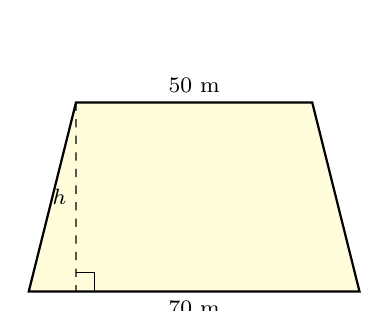
\begin{tikzpicture}[scale=0.06, font=\footnotesize]
  \coordinate (A) at (10,40);
  \coordinate (B) at (60,40);
  \coordinate (C) at (70,0);
  \coordinate (D) at (0,0);
  \draw[thick, fill=yellow!15] (A) -- (B) -- (C) -- (D) -- cycle;
  \draw[dashed] (A) -- (10,0) node[midway, left] {$h$};
  \draw (10,4) -- (14,4) -- (14,0);
  \node[above] at (35,40) {$50\text{ m}$};
  \node[below] at (35,0) {$70\text{ m}$};
\end{tikzpicture}
\end{center}
\begin{enumerate}[label=\textbf{\alph*)}, leftmargin=0.8cm, itemsep=2pt]
\item (0,5 điểm) Tính diện tích của mảnh đất?
\item (0,5 điểm) Người ta trồng ngô trên miếng đất này, mỗi mùa cứ $3\text{ ha}$ thu được $13{,}5\text{ tấn ngô}$. Hỏi trên mảnh đất này, mỗi mùa người ta thu được tất cả bao nhiêu kg ngô?
\end{enumerate}
\end{ex}
\vspace{1.5mm}


\begin{center}
\rule{4cm}{0.4pt}\\
\textit{--- HẾT ---}
\end{center}
\end{document}
